\chapter{基于软硬协同的中断响应和任务调度实现}

本章根据第三章所述的任务模型和设计方案,在 FPGA 平台上实现了上述的具备中断处理、任务通信以及任务调度的控制器(TAIC,Task Aware Interrupt Controller),并且进行了相关的软件适配,实现了基于软硬协同的中断响应和任务调度机制的系统原型。

\section{系统整体结构}

图 \ref{figure:arch} 给出了基于软硬协同的中断响应和任务调度系统的整体架构。系统由 CPU、TAIC 和外部设备三部分组成。外部设备的中断信号连接到 TAIC 的中断处理模块中,TAIC 内部维护了若干套用于不同的地址空间和特权级下的队列资源(包括就绪队列、外部中断能力槽、接收能力槽和发送能力槽),不同的队列资源之间通过任务通信模块构建硬件的通信通道。CPU、TAIC 与外部设备通过总线相连。运行于 CPU 上的处于不同地址空间和特权级之间的任务通过软硬件交互接口使用 TAIC 提供的中断处理、任务调度和任务通信功能。

\begin{figure}[htbp]
  \centering
  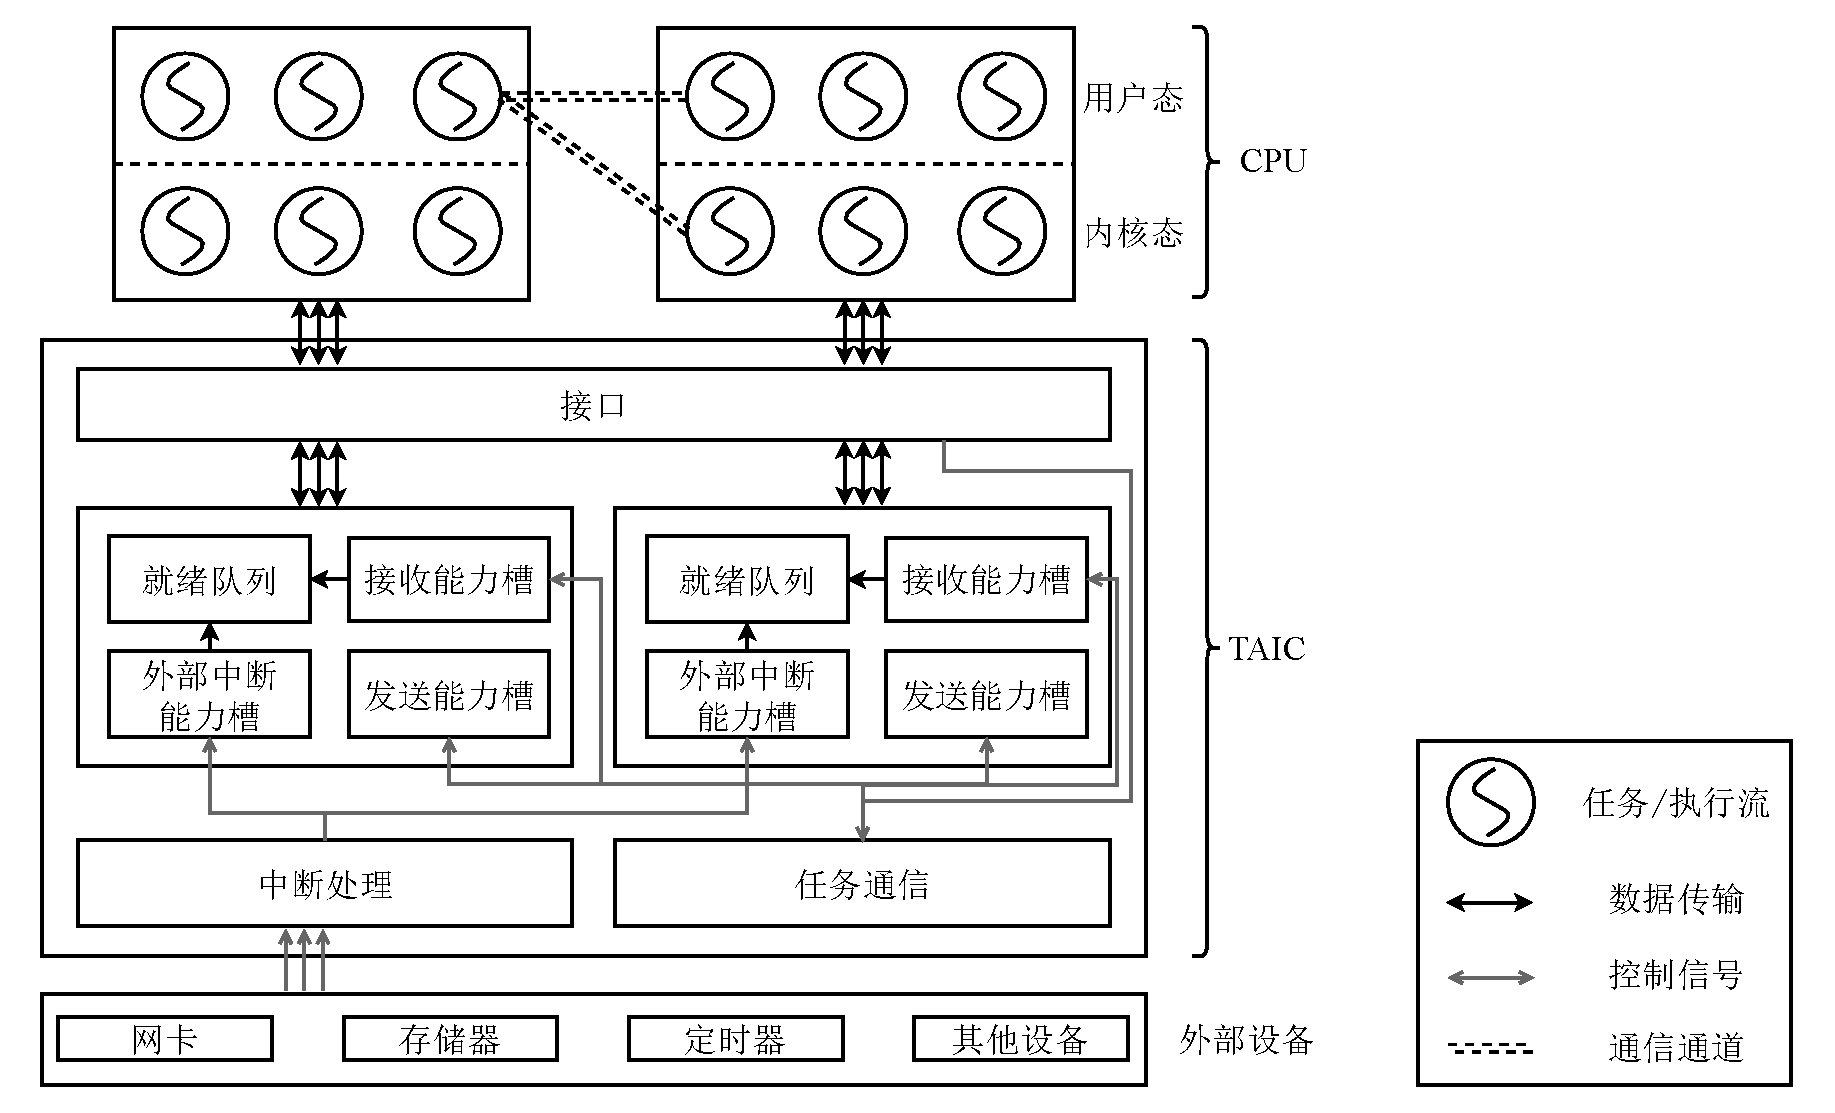
\includegraphics[width=0.8\textwidth]{figures/pdfs/arch.pdf}
  \caption{基于软硬协同的中断响应和任务调度系统整体架构}
  \label{figure:arch}
\end{figure}

\section{控制器实现}

根据 TAIC 提供的功能划分,TAIC 由四个模块构成:任务调度、中断处理、任务通信和队列资源分配与回收。

\subsection{任务调度}

TAIC 内部维护了若干任务队列,并且 TAIC 能够在不同的任务队列之间迁移任务标识,维持任务队列的偏序关系,以此来向软件提供任务调度的功能。

其中就绪队列的实现直接在硬件层面提供了软件中的任务队列所需要的出队、入队、优先级排序和负载均衡等功能,能够满足软件的任务调度需求。就绪队列由一块脉冲阵列和若干个局部队列元信息组成,如图 \ref{figure:ready_queue} 所示。

\begin{figure}
  \centering
  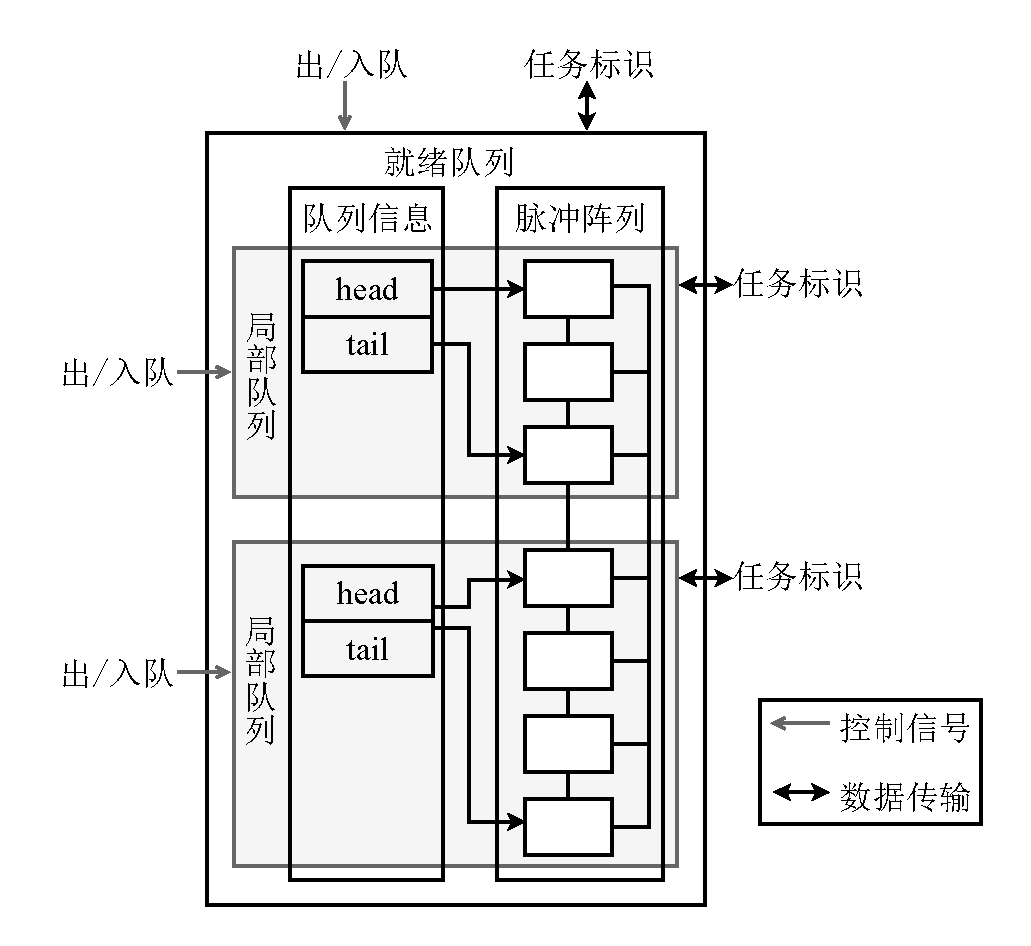
\includegraphics[width=\textwidth]{figures/pdfs/ready_queue.pdf}
  \caption{就绪队列}
  \label{figure:ready_queue}
\end{figure}

脉冲阵列用于存放任务标识,当需要删除某个位置的任务标识时,该位置后的所有任务标识自动前移即可完成删除操作;当需要在某个位置插入任务标识时,先将该位置包括后续的所有任务标识后移,然后再将任务标识插入到该位置即可完成插入操作。

基于脉冲阵列,只需要记录队列在脉冲阵列中的头部 $head$ 和尾部 $tail$ 位置即可实现局部队列。由于局部队列共用同一块脉冲阵列,因此当某个局部队列在进行出/入队操作时,位于该局部队列后的所有局部队列的 $head$ 和 $tail$ 指针都需要更新。局部队列支持的操作为:

\begin{itemize}
  \item 出队:取出脉冲阵列中 $head$ 处的任务标识,将自己的 $tail$ 指针 -1,将后续所有局部队列的 $head$ 和 $tail$ 指针 -1;
  \item 入队:将任务标识插入到脉冲阵列中 $tail$ 处,将自己的 $tail$ 指针 +1,将后续所有局部队列的 $head$ 和 $tail$ 指针 +1;
\end{itemize}

这些局部队列共同组成了一个就绪队列(全局队列),既可以单独对局部队列执行出/入队操作,也可以对全局队列执行出/入队操作。全局队列的容量存在上限(脉冲阵列可以存放的任务标识的数量),但局部队列的容量没有固定上限,当全局队列达到容量上限时,对任意局部队列进行的入队操作将会失败,无法插入任务标识。局部队列在执行出队操作时集成了负载均衡的功能,当某个局部队列为空时,会从其他具有任务的局部队列中窃取任务标识(窃取的顺序为局部队列的 $head$ 指针指向的脉冲阵列位置的顺序);只有当整个全局队列为空时,才会返回空值。

基于局部队列的窃取机制以及窃取的顺序,整个全局队列可以当作优先级队列使用,其中每个局部队列中存放优先级相同的任务标识,并且按照先进先出的规则进行排序。不同的局部队列的优先级不同,$head$ 指针在脉冲阵列的位置越靠前,优先级越高。

基于上述的就绪队列实现,软件可以灵活地使用局部队列和全局队列,已实现不同的调度策略,并且减少因为固定局部队列容量导致的硬件资源的浪费。

由于硬件资源有限,阻塞队列只用于保存因为等待外部设备以及等待任务通信而进入阻塞状态的任务的标识,对应的实现为外部中断能力槽和接收能力槽,分别在 \ref{section:interrupt} 和 \ref{section:communication} 中描述。

\subsection{中断处理}
\label{section:interrupt}

TAIC 快速处理中断机制依赖于任务队列中的维护的外部中断能力槽,它记录了由于等待外部设备中断而进入阻塞状态的任务的标识。由于应用程序通常只有一个任务用于处理外部中断,因此,针对每个外部中断信号只准备了一个槽位。其结构以及处理流程如图 \ref{figure:extintr} 所示。

\begin{figure}[htbp]
  \centering
  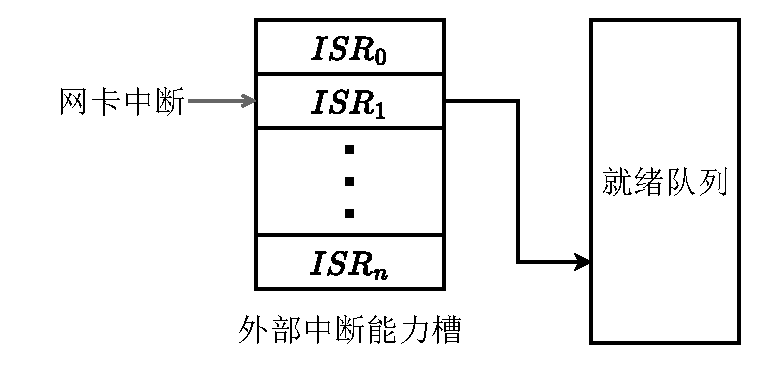
\includegraphics[width=0.8\textwidth]{figures/pdfs/extintr.pdf}
  \caption{外部中断处理}
  \label{figure:extintr}
\end{figure}

$ISR_{i}$ 表示与中断号为 $i$ 相关的任务标识,在使用硬件快速处理中断能力时,需要软件向外部中断能力槽中注册任务标识(该任务为阻塞状态),注册成功即为使能了硬件外部中断处理机制。当外部设备产生中断信号时,TAIC 的中断处理模块会根据中断信号来检查对应的槽位,若其中存在任务标识,将任务标识从槽中取出,并放入到就绪队列中的合适位置,以此来唤醒因为等待外部设备中断而进入阻塞状态的任务。一旦完成唤醒操作,外部中断能力槽中该中断对应的槽位会被清空,TAIC 的快速处理该中断的能力会被屏蔽,直到软件再次注册该中断的处理任务重新使能该机制。

此外,若中断的处理任务的优先级较高,TAIC 会向 CPU 发送中断信号,CPU 在收到中断信号后,直接进行任务切换。TAIC 的硬件快速处理中断机制可以无视特权级,可以在用户态使用,但需要额外的机制来保证任意时刻只有一个进程或内核在使用同一个外部设备。但对于某些特殊的应用场景,例如在虚拟化场景中,多个内核使用同一个硬件定时器,则可以通过 TAIC 来实现时钟设备的虚拟化。

\subsection{任务通信}
\label{section:communication}

由于任务通信的发送方和接收方是处于不同地址空间和特权级下的任务,而进程可以用于区分地址空间和特权级,且进程属于操作系统,因此使用操作系统标识和进程标识来表示任务所出的环境。因此,TAIC 基于操作系统标识和进程标识,在内部维护了若干的发送能力槽和接收能力槽,用于构建硬件支持的跨越不同环境的任务通信通道。

发送能力槽中记录了当前环境下,可以向哪些接收方 $(recv\_os_{i}, recv\_proc_{j})$ 发起通信以及通信通道的编号$irq_{k}$,而接收能力槽则记录了当前环境下能够接收哪些发送方 $(send\_os_{l}, send\_proc_{m})$的通信请求、通信通道编号 $irq_{n}$,并且记录了当前环境下因为等待任务通信而进入阻塞状态的任务标识 $isr_{x}$。发送能力槽和接收能力槽的结构以及任务通信流程如图 \ref{figure:communication} 所示。

\begin{figure}[htbp]
  \centering
  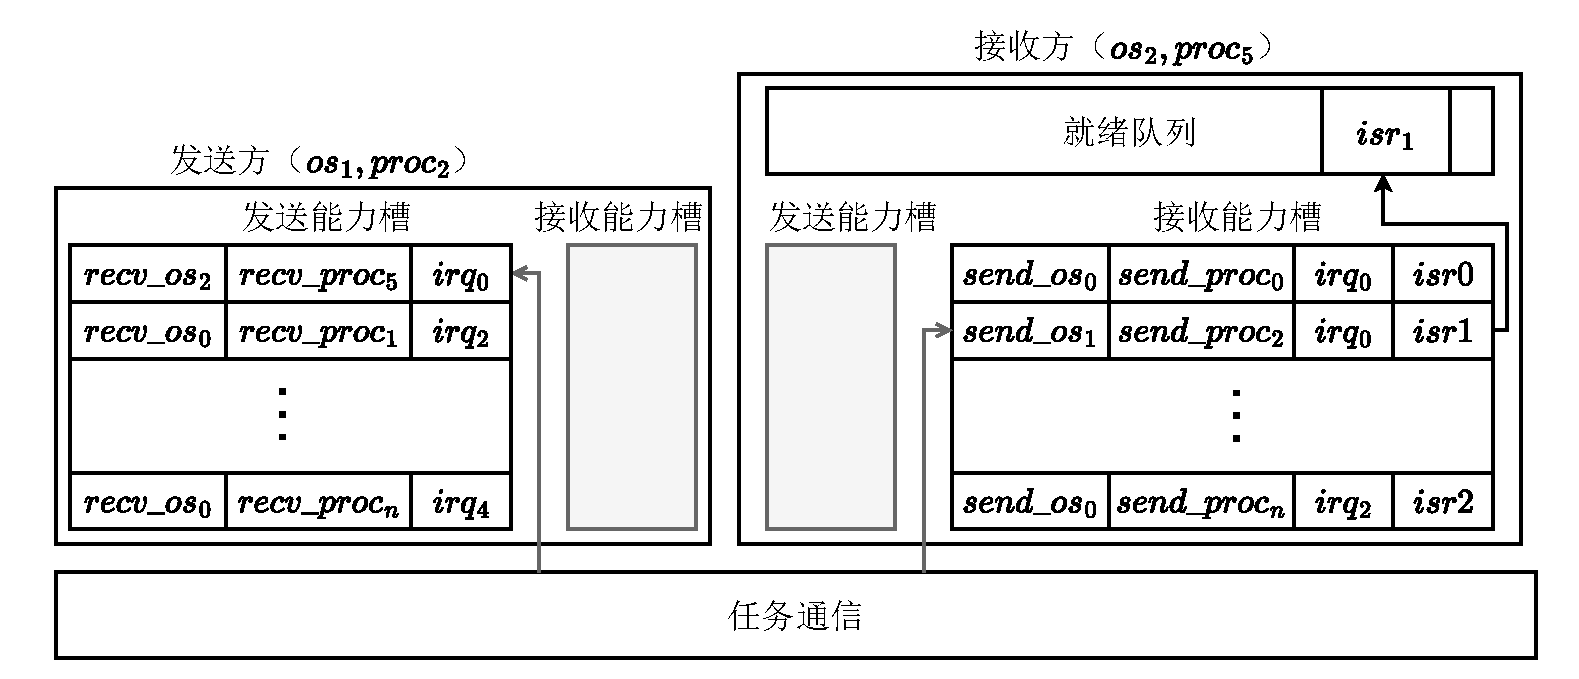
\includegraphics[width=\textwidth]{figures/pdfs/communication.pdf}
  \caption{任务通信}
  \label{figure:communication}
\end{figure}

在使用硬件支持的任务通信能力时,发送方需要向发送能力槽中写入接收方的操作系统标识和进程标识,以及通信通道的编号,注册成功即为使能了发送能力。接收方需要向接收能力槽中写入发送方的操作系统标识和进程标识、通信通道的编号以及任务标识,注册成功即为使能了接收能力。

发送方通过向 TAIC 的端口中写入接收方的操作系统标识、进程标识以及通信通道编号来发起通信,TAIC 的任务通信模块根据发送方提供的标识信息,首先检查发送方的发送能力槽中是否存在对应的条目,如果不存在,则通信失败;若存在条目,任务通信模块根据发送能力槽条目中记录的接收方的操作系统标识、进程标识以及通信通道标识,检查接收方的接收能力槽中是否存在对应的条目,如果不存在,则通信失败;如果存在,任务通信模块将接收能力槽中对应的条目清除,将等待通信的任务标识放入到就绪队列中的合适位置,完成任务通信。若唤醒的接收方任务的优先级较高,TAIC 会向 CPU 发送中断信号,CPU 在收到中断信号后,直接进行任务切换。

\subsection{资源分配与回收}

每套资源由就绪队列、外部中断能力槽、发送能力槽和接收能力槽组成,向位于特定地址空间和特权级下的软件提供任务调度、中断处理和任务通信功能。由于操作系统与进程可以用于区分地址空间和特权级,因此本文使用操作系统和进程的标识符 $(os\_id, proc\_id)$ 来区分不同的资源,软件要使用这些功能时,需要向 TAIC 的资源分配接口写入操作系统标识和进程标识,TAIC 会根据这些标识符来分配相应的资源,最终返回软件可以操作的句柄。资源分配的流程如下:

\begin{enumerate}
  \item 向 TAIC 的资源分配接口依次写入 $os\_id$ 和 $proc\_id$。
  
  \item TAIC 根据 $os\_id$ 和 $proc\_id$ 查找是否已经分配了对应的资源,若没有,则分配一套资源,将其标记为 $(os\_id, proc\_id)$ 已使用,并在资源初始化之后执行 \ref{item:alloc_handle};若已经分配,则执行 \ref{item:alloc_handle};如果控制器中没有空闲资源,则分配失败。
  
  \item \label{item:alloc_handle} 分配软件操作句柄,句柄包括了对这套资源中的就绪队列中的某个局部队列、外部中断能力槽、发送能力槽和接收能力槽的操作接口。
\end{enumerate}

在相同的地址空间和特权级 $(os\_id, proc\_id)$ 中,不同的句柄对中断处理、任务通信等接口的操作是等价的,都会对外部中断能力槽、发送能力槽和接收能力槽产生相同的影响,但对就绪队列中的局部队列的操作是不同的,这是为了保证软件在使用这些接口时是一致的。

资源回收的流程如下:

\begin{enumerate}
  \item 向 TAIC 的资源回收接口依次写入 $os\_id$ 和 $proc\_id$。
  
  \item TAIC 根据 $os\_id$ 和 $proc\_id$ 查找是否已经分配了对应的资源,若没有,则回收失败;若已经分配,则执行 \ref{item:free_handle}。
  
  \item \label{item:free_handle} 回收软件操作句柄,释放软件对该句柄对应的局部队列的操作权限。若这套资源所有申请的操作句柄都被回收时,将资源标记为未使用。
\end{enumerate}

\section{任务抢占}

TAIC 提供了中断处理和任务通信的能力,硬件直接唤醒了对应的阻塞任务,但这不意味着被唤醒的任务会马上执行,若 CPU 上正存在其他的任务执行,而被唤醒的任务优先级较高,则会导致被唤醒任务的响应延时增加。因此,TAIC 会在被唤醒的任务优先级较高时,向 CPU 发送中断,实现了抢占式任务调度。由于被唤醒的任务可能处于内核态或用户态,因此 TAIC 根据被唤醒的任务标识中的操作系统标识和进程标识来判断任务所处的特权级,向 CPU 发送不同的中断信号。因此需要实现用户态中断扩展。本文在 rocket-chip 软核 \cite{rocket-chip} 上增加了用户态中断相关的控制寄存器以及 $uret$ 指令,并且将 TAIC 的中断信号与 CPU 的 $mip$ 寄存器的 $SSIP$ 和 $USIP$ 位相连,实现了 RISC-V 的 N 扩展。

当被唤醒的任务处于内核态且优先级较高时,TAIC 会产生中断信号,将 $mip$ 寄存器的 $SSIP$ 位拉高,CPU 跳转至内核态的中断向量寄存器 $stvec$ 指向的位置,保存被打断任务的寄存器现场,从 TAIC 中取出被唤醒的任务标识并执行任务,从而减少响应延时。

当被唤醒的任务处于用户态,这里的处理比唤醒处于内核态的任务更加复杂。可以分为两类:

\begin{enumerate}
  \item \label{item:uintr_online} 当 CPU 正在运行与被唤醒任务处于相同进程和特权级下的其他任务,若被唤醒任务的优先级较高,则 TAIC 会产生中断信号,将 $mip$ 寄存器的 $USIP$ 位拉高,CPU 跳转至用户态的中断向量寄存器 $utvec$ 指向的位置,保存被打断任务的寄存器现场,从 TAIC 中取出被唤醒的任务标识并执行任务,从而减少响应延时。
  \item 若当前 CPU 正在执行其他的与被唤醒任务处于不同地址空间或不同特权级的任务时,TAIC 会暂时挂起这次唤醒所产生的中断,直到 CPU 再次回到 \ref{item:uintr_online} 这种情况。
\end{enumerate}

\begin{figure}[htbp]
  \centering
  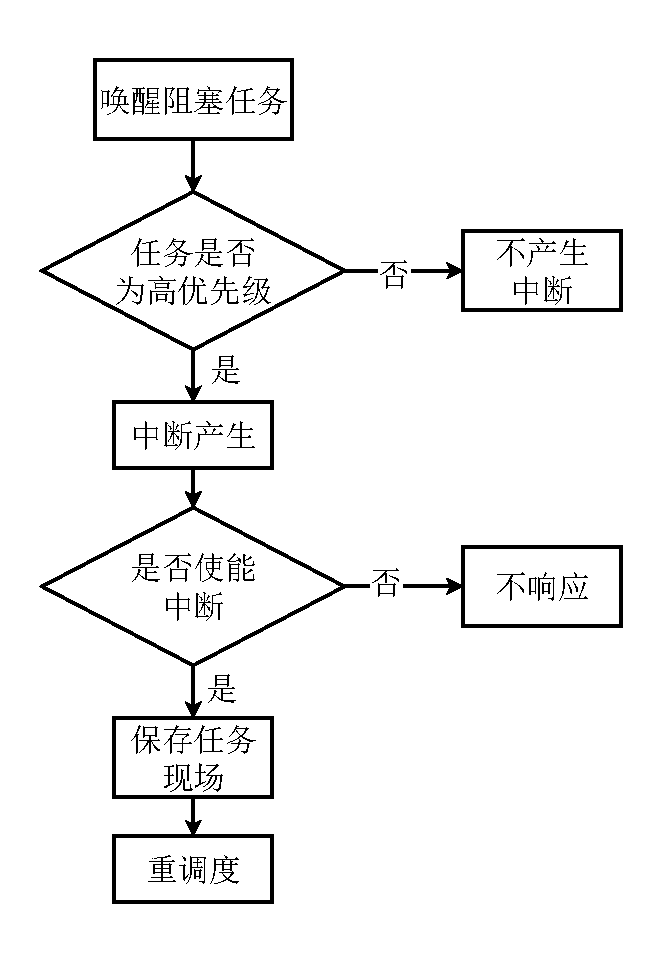
\includegraphics[width=0.6\textwidth]{figures/pdfs/userintr.pdf}
  \caption{任务抢占的流程}
  \label{figure:userintr}
\end{figure}

\section{软件适配}

TAIC 可以与现有的进程、线程或协程任务模型进行结合,线程与协程模型建立在进程提供的地址空间隔离机制上,将 TAIC 的端口映射到各自的地址空间中,即可向 TAIC 申请硬件资源用于任务调度、中断处理和任务通信。软件与 TAIC 的交互通过申请获取的硬件资源句柄进行。

\subsection{申请硬件资源}

TAIC 中的硬件资源通过操作系统标识和进程标识进行区分,因此在申请使用 TAIC 的硬件资源时,需要向资源分配端口写操作系统标识 $os\_id$ 和进程标识 $pid$。在内核中使用 TAIC 时,$os\_id$ 为一个固定的数值 $OSID$(由内核在初始化时进行约定),$pid$ 为 0,因此,内核向 TAIC的资源分配接口写入 $(OSID, 0)$ 即可使用 TAIC 提供的功能。在用户态使用时,则需要通过 \verb|get_taic_handle| 系统调用,该系统调用首先向 TAIC 的资源分配端口写入 $(OSID, pid)$ 申请资源句柄,并将资源句柄对应的端口映射到用户进程的地址空间中,最终将资源句柄返回给用户态,对应的伪代码为 \ref{alg:get_taic_handler}。

\floatname{algorithm}{系统调用}
\begin{algorithm}[!ht]
  \caption{get\_taic\_handler}
  \label{alg:get_taic_handler}
  \begin{algorithmic}[1]
    \Require
    \Ensure handler
    
    \State  pid \gets get\_pid()
    \State  osid \gets OSID
    \State  taic\_base \gets TAIC\_BASE
    \State  size \gets HANDLER\_SIZE
    \State  handler\_id \gets taic\_alloc(osid, pid) {\Comment{申请 TAIC 资源,获取资源编号}}
    \If {handler\_id = $0$}
        \State  handler \gets $-1$
        \Return handler
    \EndIf
    \State handler\_addr \gets handler\_addr(handler\_id, 
    \Statex \qquad \qquad \qquad \qquad \qquad \qquad taic\_base) {\Comment{根据 TAIC 基址和资源编号,获取资源基址}}
    \State mem\_fd \gets open(\textquotedbl/dev/mem\textquotedbl, O\_RDWR)

    \If {mem\_fd = $-1$}
        \State taic\_free(handler\_id)
        \State handler \gets $-1$
        \Return handler
    \EndIf
    \State handler \gets mmap(NULL, size, 
    \Statex \qquad \qquad \qquad \qquad PROT\_READ | PROT\_WRITE, 
    \Statex \qquad \qquad \qquad \qquad MAP\_SHARED, 
    \Statex \qquad \qquad \qquad \qquad mem\_fd, handler\_addr) {\Comment{将 TAIC 资源句柄映射到进程地址空间中}}
    \If {handler = NULL}
        \State taic\_free(handler\_id)
        \State  handler = $-1$
    \EndIf
    \Return handler
  \end{algorithmic}
\end{algorithm}

\subsection{任务通信}

当两个进程中的接收方申请到 TAIC 的硬件资源 $handler$ 后,可以通过 \verb|task_enqueue(handler, task_id)| 和 \verb|task_dequeue(handler)| 进行任务调度,并且基于 TAIC 直接通信。伪代码 \ref{alg:communication} 展示了两个进程单向通信的示例。同理,双向通信只需要两个进程都注册发送和接收能力即可。

\floatname{algorithm}{单向通信示例}
\begin{algorithm}[!ht]
  \caption{communication\_example}
  \label{alg:communication}
  \begin{algorithmic}[1]
    \State send\_pid, recv\_pid, irq, os\_id, is\_inited, has\_received

    \Procedure{Sender}{}      \Comment{发送方}
      \State send\_pid \gets sys\_get\_pid()
      \State send\_handler \gets get\_taic\_handler() \Comment{获取 TAIC 资源句柄}
      \State register\_sender(send\_handler, os\_id, recv\_pid, irq) \Comment{注册发送能力}
      \Loop
        \While {is\_inited = false}
        \EndWhile
        \State is\_inited \gets false
        \State send(send\_handler, os\_id, recv\_pid, irq) \Comment{发送方发送通知}
        \While {has\_received = false}
        \EndWhile
        \State has\_received \gets false
      \EndLoop
    \EndProcedure

    \Procedure{Receiver}{}      \Comment{接收方}
      \State recv\_pid \gets sys\_get\_pid()
      \State recv\_handler \gets get\_taic\_handler() 
      \Loop
        \State register\_receiver(recv\_handler, os\_id, send\_pid, irq, handle\_task) \Comment{注册接收能力}
        \State is\_inited \gets true
        \State task\_id \gets task\_dequeue(recv\_handler)
        \While {task\_id = $0$} \Comment{等待收到通知}
          \State task\_id \gets task\_dequeue(recv\_handler)
        \EndWhile
        \State has\_received \gets true
      \EndLoop
    \EndProcedure

    \Procedure{handle\_task}{}      \Comment{等待通知的任务}
      \State xxxx
    \EndProcedure
  \end{algorithmic}
\end{algorithm}

当接收方处于用户态且优先级较高时,为了减少任务的响应延时,需要初始化并使能用户态中断。在收到用户态中断时,进行重调度,伪代码如 \ref{alg:uintr} 所示。

\floatname{algorithm}{用户态中断初始化}
\begin{algorithm}[!ht]
  \caption{user\_intr\_init}
  \label{alg:uintr}
  \begin{algorithmic}[1]
    \State taic\_handler
    \Function{user\_intr\_init}{}
      \State csr\_write(CSR\_UTVEC, uintr\_entry) \Comment{设置用户态中断入口}
      \State csr\_set(CSR\_USTATUS, USTATUS\_UIE) \Comment{使能用户态中断}
      \State csr\_set(CSR\_UIE, MIE\_USIE) \Comment{使能用户态中断}
    \EndFunction

    \Function{uintr\_entry}{}
      \State xxxx \Comment{保存被打断任务的上下文}
      \State task\_id \gets task\_dequeue(taic\_handler) \Comment{取出被唤醒的任务标识}
      \State switch\_to\_task(task\_id) \Comment{切换到被唤醒的任务}
    \EndFunction
  \end{algorithmic}
\end{algorithm}

\section{本章小结}

本章给出了基于软硬协同的中断响应和任务调度系统的整体架构,详细描述了 TAIC 内部各个模块的设计和实现,包括就绪队列、外部中断能力槽、发送能力槽和接收能力槽,解释了它们如何在硬件层面提供软件需要的能力。并且,本章描述了 TAIC 如何与已有的中断机制结合,实现任务抢占。最后给出了如何在现有的软件中使用 TAIC 提供的硬件加速能力的伪代码示例,验证了第三章设计方案的可行性。
